% ASSERT_CONVENTION: natural_units=natural, metric_signature=mostly_minus, fourier_convention=physics, coupling_convention=alpha_s, generator_normalization=T(fund)=1/2, covariant_derivative_sign=D_mu=partial_mu-igA
%
% Exercise Set 2: The Conformal Window
% Part of: The Dualised Standard Model -- Part III Lecture Notes
% Convention: b_0 = (11N_c - 2N_f)/3 for N_f Dirac flavours, T(fund) = 1/2
%
\documentclass[11pt,a4paper]{article}
% ASSERT_CONVENTION: natural_units=natural, metric_signature=mostly_minus, fourier_convention=physics, coupling_convention=alpha_s, generator_normalization=T(fund)=1/2, covariant_derivative_sign=D_mu=partial_mu-igA
%
% CONVENTIONS (Seiberg hep-th/9411149)
% Metric: (+,-,-,-) (mostly minus)
% T(fund) = 1/2 per Weyl fermion
% b_0 = (11N_c - 2N_f)/3 for N_f Dirac flavours
% D_mu = partial_mu - ig A_mu^a T^a
% A(fund) = 1 (cubic anomaly coefficient per fundamental Weyl fermion)
% alpha_s = g_s^2 / (4 pi)
% R[Q] = (N_f - N_c)/N_f; R[W] = 2
% N_f counts Dirac flavour pairs (each = 2 Weyl fermions)
%
% This file is \input{} by all lecture files.

%% ---------- Document class ----------
% (loaded by the wrapper; preamble only provides packages and macros)

%% ---------- Standard packages ----------
\usepackage{amsmath,amssymb,amsthm,mathtools}
\usepackage{hyperref}
\usepackage[capitalise,noabbrev]{cleveref}
\usepackage{enumitem}
\usepackage{booktabs}
\usepackage{array}
\usepackage{xcolor}
\usepackage{tikz}
\usetikzlibrary{arrows.meta,decorations.markings,positioning,calc}
\usepackage{fancybox}
\usepackage{tcolorbox}
\tcbuselibrary{skins,breakable}
\usepackage{slashed}              % Feynman slash notation
\usepackage{cite}                 % compressed citation lists

%% ---------- Hyperref configuration ----------
\hypersetup{
  colorlinks=true,
  linkcolor=blue!70!black,
  citecolor=green!50!black,
  urlcolor=blue!80!black,
  pdfauthor={Part III Lecture Notes},
  pdftitle={The Dualised Standard Model}
}

%% ---------- Theorem environments ----------
\theoremstyle{plain}
\newtheorem{theorem}{Theorem}[section]
\newtheorem{lemma}[theorem]{Lemma}
\newtheorem{proposition}[theorem]{Proposition}
\newtheorem{corollary}[theorem]{Corollary}

\theoremstyle{definition}
\newtheorem{definition}[theorem]{Definition}
\newtheorem{example}[theorem]{Example}
\newtheorem{exercise}{Exercise}[section]

\theoremstyle{remark}
\newtheorem{remark}[theorem]{Remark}

%% ---------- Physics macros: gauge groups and representations ----------
\newcommand{\Nc}{N_{\!c}}
\newcommand{\Nf}{N_{\!f}}
\newcommand{\SU}[1]{\mathrm{SU}(#1)}
\newcommand{\UU}[1]{\mathrm{U}(#1)}

% Representations
\newcommand{\fund}{\square}
\newcommand{\antifund}{\overline{\square}}
\newcommand{\adj}{\mathrm{adj}}
\newcommand{\antisym}{\wedge^{\!2}}        % antisymmetric rank-2
\newcommand{\sym}{\mathrm{S}_2}           % symmetric rank-2

%% ---------- Physics macros: group theory constants ----------
% Dynkin index: Tr(T^a T^b) = T(R) delta^{ab}
\newcommand{\Tfund}{\tfrac{1}{2}}          % T(fund) = 1/2 per Weyl fermion
\newcommand{\Tadj}{\Nc}                    % T(adj) = N_c
\newcommand{\Cfund}{\frac{\Nc^2 - 1}{2\Nc}}  % C_2(fund)
\newcommand{\Cadj}{\Nc}                    % C_2(adj)

% Cubic anomaly coefficient: A(R) = Tr_R[T^a {T^b, T^c}] with A(fund) = 1
\newcommand{\Afund}{1}

%% ---------- Physics macros: beta function ----------
\newcommand{\bzero}{b_0}
\newcommand{\bone}{b_1}
\newcommand{\alphas}{\alpha_s}
\newcommand{\gs}{g_s}

%% ---------- Physics macros: SUSY / R-charge ----------
\newcommand{\Rcharge}[1]{R[#1]}
\newcommand{\Wsup}{W}                      % superpotential

%% ---------- Physics macros: covariant derivative and field strength ----------
\newcommand{\Dmu}{D_\mu}
\newcommand{\Fmn}{F_{\mu\nu}}
\newcommand{\Ftilde}{\widetilde{F}_{\mu\nu}}

%% ---------- Physics macros: common abbreviations ----------
\newcommand{\ie}{\textit{i.e.}}
\newcommand{\eg}{\textit{e.g.}}
\newcommand{\cf}{\textit{cf.}}
\newcommand{\IR}{\ensuremath{\mathrm{IR}}}
\newcommand{\UV}{\ensuremath{\mathrm{UV}}}
\newcommand{\AF}{\ensuremath{\mathrm{AF}}}
\newcommand{\BZ}{\ensuremath{\mathrm{BZ}}}
\newcommand{\NSVZ}{\ensuremath{\mathrm{NSVZ}}}
\newcommand{\SQCD}{\ensuremath{\mathrm{SQCD}}}
\newcommand{\QCD}{\ensuremath{\mathrm{QCD}}}
\newcommand{\SM}{\ensuremath{\mathrm{SM}}}
\newcommand{\Tr}{\mathrm{Tr}}

%% ---------- Convention box macro ----------
\newtcolorbox{conventionbox}[1][]{%
  enhanced,
  colback=blue!5!white,
  colframe=blue!60!black,
  fonttitle=\bfseries,
  title={Conventions},
  #1
}

%% ---------- Comparison table style ----------
\newtcolorbox{comparisontable}[1][]{%
  enhanced,
  colback=orange!5!white,
  colframe=orange!70!black,
  fonttitle=\bfseries,
  title={Comparison},
  #1
}

%% ---------- Warning / important box ----------
\newtcolorbox{warningbox}[1][]{%
  enhanced,
  colback=red!5!white,
  colframe=red!70!black,
  fonttitle=\bfseries,
  title={Important},
  #1
}

%% ---------- Preview / forward-reference box ----------
\newtcolorbox{previewbox}[1][]{%
  enhanced,
  colback=green!5!white,
  colframe=green!50!black,
  fonttitle=\bfseries,
  title={Preview},
  #1
}

%% ---------- Page layout ----------
\usepackage[margin=2.5cm]{geometry}
\setlength{\parskip}{0.4em}
\setlength{\parindent}{0em}

%% ---------- Section formatting ----------
\usepackage{titlesec}
\titleformat{\section}{\Large\bfseries}{\thesection}{1em}{}
\titleformat{\subsection}{\large\bfseries}{\thesubsection}{1em}{}

%% ---------- End of preamble ----------


\title{\textbf{Exercise Set 2: The Conformal Window}}
\author{The Dualised Standard Model --- Part III Exercises}
\date{Lent Term 2027}

\begin{document}
\maketitle

\begin{conventionbox}[title={Conventions for these exercises}]
\renewcommand{\arraystretch}{1.3}
\begin{tabular}{@{}l l@{}}
\toprule
\textbf{Quantity} & \textbf{Convention} \\
\midrule
Beta function & $\mu\,d\alphas/d\mu = -(\bzero/2\pi)\,\alphas^2
  - (\bone/4\pi^2)\,\alphas^3 + \cdots$ \\
One-loop coefficient & $\bzero = (11\Nc - 2\Nf)/3$ for $\Nf$ Dirac flavours \\
Dynkin index & $T(\fund) = \Tfund$, $T(\adj) = \Nc$ \\
$R$-charge & $\Rcharge{Q} = (\Nf - \Nc)/\Nf$; $\Rcharge{\Wsup} = 2$ \\
SUSY conformal window & $3\Nc/2 < \Nf < 3\Nc$ (exact, Seiberg) \\
\bottomrule
\end{tabular}

\medskip

\noindent References: Lecture~1, \S\ref*{sec:conformal}.
\end{conventionbox}

\bigskip

%% ========================================================================
%%  PROBLEM 1: Beta function coefficient survey (warm-up)
%% ========================================================================
\section*{Problem 1: Beta function coefficient survey
  \hfill $\star$ \normalsize(15 min)}
\addcontentsline{toc}{section}{Problem 1: Beta function coefficient survey}
\label{prob:b0-survey}

\noindent\textbf{Background.}
The one-loop beta function coefficient $\bzero$ determines whether a gauge
theory is asymptotically free ($\bzero > 0$) and sets the scale for the
conformal window.

\medskip
\noindent\textbf{Questions.}
\begin{enumerate}[label=(\alph*)]
  \item Compute $\bzero = (11\Nc - 2\Nf)/3$ for $\SU{3}$ gauge theory
    with the following numbers of Dirac flavours:

    \begin{center}
    \renewcommand{\arraystretch}{1.2}
    \begin{tabular}{@{}l l l@{}}
    $\Nf = 0$ & (pure Yang--Mills) & $\bzero = ?$ \\
    $\Nf = 2$ & (2-flavour QCD) & $\bzero = ?$ \\
    $\Nf = 6$ & (6-flavour QCD) & $\bzero = ?$ \\
    $\Nf = 16$ & (near AF boundary) & $\bzero = ?$ \\
    $\Nf = 17$ & (above AF boundary) & $\bzero = ?$ \\
    \end{tabular}
    \end{center}

  \item For each case, state whether the theory is asymptotically free.

  \item \textbf{Convention check.} Verify that the formula
    \begin{equation}
      \bzero = \frac{11}{3}\,T(\adj) - \frac{4}{3}\,\Nf\,T(\fund)
    \end{equation}
    with $T(\fund) = 1/2$ and $T(\adj) = \Nc$ gives the same result as
    $\bzero = (11\Nc - 2\Nf)/3$.
\end{enumerate}

\bigskip
\hrule
\bigskip

\begin{proof}[\textbf{Solution to Problem 1}]

\textbf{(a)} Using $\bzero = (11\Nc - 2\Nf)/3$ with $\Nc = 3$:

\begin{center}
\renewcommand{\arraystretch}{1.3}
\begin{tabular}{@{}c l c c@{}}
\toprule
$\Nf$ & Description & $\bzero = (33 - 2\Nf)/3$ & AF? \\
\midrule
$0$ & Pure Yang--Mills & $(33-0)/3 = 11$ & Yes \\
$2$ & 2-flavour QCD & $(33-4)/3 = 29/3$ & Yes \\
$6$ & 6-flavour QCD & $(33-12)/3 = 7$ & Yes \\
$16$ & Near AF boundary & $(33-32)/3 = 1/3$ & Yes \\
$17$ & Above AF boundary & $(33-34)/3 = -1/3$ & No \\
\bottomrule
\end{tabular}
\end{center}

\textbf{(b)} The theory is asymptotically free when $\bzero > 0$, \ie\
when $\Nf < 11\Nc/2 = 33/2 = 16.5$.  So $\Nf \leq 16$ gives AF;
$\Nf \geq 17$ does not.

\medskip

\textbf{(c) Convention check.}

$\frac{11}{3}\,T(\adj) - \frac{4}{3}\,\Nf\,T(\fund)
= \frac{11}{3}\,\Nc - \frac{4}{3}\,\Nf \times \frac{1}{2}
= \frac{11\Nc}{3} - \frac{2\Nf}{3}
= \frac{11\Nc - 2\Nf}{3}$.

This is identical to $\bzero = (11\Nc - 2\Nf)/3$. \quad$\checkmark$

\medskip

\textit{Important:} The factor of 4/3 in $-\frac{4}{3}\,\Nf\,T(\fund)$
comes from the fermion loop contribution, where the 4 counts the Dirac
degrees of freedom (2 spin $\times$ 2 particle/antiparticle, or equivalently
2 Weyl fermions per Dirac pair times the factor 2 from the loop integral).
With $T(\fund) = 1/2$, the overall contribution per Dirac fermion is
$\frac{4}{3} \times \frac{1}{2} = \frac{2}{3}$.
\end{proof}

\newpage

%% ========================================================================
%%  PROBLEM 2: Banks-Zaks fixed point
%% ========================================================================
\section*{Problem 2: The Banks--Zaks fixed point
  \hfill $\star\star$ \normalsize(30 min)}
\addcontentsline{toc}{section}{Problem 2: The Banks--Zaks fixed point}
\label{prob:banks-zaks}

\noindent\textbf{Background.}
When $\Nf$ is just below the asymptotic freedom boundary $11\Nc/2$, the
one-loop coefficient $\bzero$ is small and positive.  If the two-loop
coefficient $\bone$ is negative, the two-loop beta function has a non-trivial
zero at a small coupling---the Banks--Zaks fixed point \cite{BanksZaks1982}.

\medskip
\noindent\textbf{Questions.}
\begin{enumerate}[label=(\alph*)]
  \item Write the two-loop beta function in the convention
    \begin{equation}
      \mu\frac{d\alphas}{d\mu}
      = -\frac{\bzero}{2\pi}\,\alphas^2
        - \frac{\bone}{4\pi^2}\,\alphas^3,
      \label{eq:ex-beta-2loop}
    \end{equation}
    where
    \begin{equation}
      \bone = \frac{1}{3}\Bigl[34\Nc^2
        - \Nf\Bigl(13\Nc - \frac{3}{\Nc}\Bigr)\Bigr].
      \label{eq:ex-b1}
    \end{equation}

  \item Show that setting $\beta(\alphas^*) = 0$ (with $\alphas^* \neq 0$)
    gives
    \begin{equation}
      \alphas^* = -\frac{2\pi\,\bzero}{\bone}.
      \label{eq:ex-bz-fixedpoint}
    \end{equation}
    State the conditions on $\bzero$ and $\bone$ for $\alphas^*$ to be
    physical (positive).

  \item For $\SU{3}$ with $\Nf = 16$:
    \begin{enumerate}[label=(\roman*)]
      \item Compute $\bzero$.
      \item Compute $\bone$.
      \item Compute $\alphas^*$.
      \item Is the perturbative expansion reliable?
    \end{enumerate}

  \item For $\SU{3}$ with $\Nf = 15$, repeat the computation. How does
    the reliability of the perturbative result change?

  \item Explain why $\alphas^* \to 0$ as $\Nf \to 11\Nc/2$ from below.
\end{enumerate}

\bigskip
\hrule
\bigskip

\begin{proof}[\textbf{Solution to Problem 2}]

\textbf{(a)} The two-loop beta function is
\[
  \mu\frac{d\alphas}{d\mu}
  = -\frac{\bzero}{2\pi}\,\alphas^2
    - \frac{\bone}{4\pi^2}\,\alphas^3
  + \mathcal{O}(\alphas^4),
\]
with $\bzero = (11\Nc - 2\Nf)/3$ and
$\bone = \frac{1}{3}[34\Nc^2 - \Nf(13\Nc - 3/\Nc)]$.

This is equations~(\ref*{eq:beta-2loop}) and~(\ref*{eq:b1}) of Lecture~1.

\textbf{(b)} Setting $\beta(\alphas^*) = 0$ and dividing by $\alphas^{*2}$
(since $\alphas^* \neq 0$):
\begin{align}
  0 &= -\frac{\bzero}{2\pi} - \frac{\bone}{4\pi^2}\,\alphas^*, \\
  \frac{\bone}{4\pi^2}\,\alphas^* &= -\frac{\bzero}{2\pi}, \\
  \alphas^* &= -\frac{\bzero}{2\pi} \times \frac{4\pi^2}{\bone}
  = -\frac{2\pi\,\bzero}{\bone}.
  \label{eq:bz-derivation}
\end{align}

For $\alphas^*$ to be physical (\ie\ positive), we need:
\begin{itemize}
  \item $\bzero > 0$ (asymptotic freedom), and
  \item $\bone < 0$ (so the ratio $-\bzero/\bone > 0$).
\end{itemize}

\textbf{(c) $\SU{3}$, $\Nf = 16$:}

\textbf{(i)} $\bzero = (33 - 32)/3 = 1/3$.

\textbf{(ii)} $\bone = \frac{1}{3}[34 \times 9 - 16(13 \times 3 - 3/3)]$:
\begin{align}
  34\Nc^2 &= 34 \times 9 = 306, \\
  13\Nc - \frac{3}{\Nc} &= 13 \times 3 - \frac{3}{3} = 39 - 1 = 38, \\
  \Nf \times 38 &= 16 \times 38 = 608, \\
  \bone &= \frac{306 - 608}{3} = \frac{-302}{3}.
\end{align}
So $\bone = -302/3 < 0$. \quad$\checkmark$

\textbf{(iii)}
\begin{align}
  \alphas^* &= -\frac{2\pi \times (1/3)}{(-302/3)}
  = -\frac{2\pi/3}{-302/3}
  = \frac{2\pi}{302}
  \approx 0.0208.
\end{align}

\textbf{(iv)} Since $\alphas^* \approx 0.021 \ll 1$, the perturbative
expansion is \emph{reliable}.  Higher-loop corrections are suppressed by
powers of $\alphas^*/(4\pi) \sim 0.002$ and are negligible.  The
Banks--Zaks fixed point is under perturbative control.

\bigskip

\textbf{(d) $\SU{3}$, $\Nf = 15$:}

$\bzero = (33 - 30)/3 = 1$.

$\bone$: $13\Nc - 3/\Nc = 38$ (same as before). $\Nf \times 38 = 15 \times 38 = 570$.
\begin{align}
  \bone &= \frac{306 - 570}{3} = \frac{-264}{3} = -88.
\end{align}

\begin{align}
  \alphas^* &= -\frac{2\pi \times 1}{-88}
  = \frac{2\pi}{88}
  = \frac{\pi}{44}
  \approx 0.071.
\end{align}

This is larger than the $\Nf = 16$ case but still reasonably small
($\alphas^*/(4\pi) \approx 0.006$).  The perturbative result is
\emph{marginally reliable}---higher-loop corrections may contribute at the
10--20\% level, but the qualitative conclusion (an IR fixed point exists)
is robust.

\textbf{Comparison:}

\begin{center}
\renewcommand{\arraystretch}{1.3}
\begin{tabular}{@{}c c c c c@{}}
\toprule
$\Nf$ & $\bzero$ & $\bone$ & $\alphas^*$ & Reliability \\
\midrule
$16$ & $1/3$ & $-302/3$ & $2\pi/302 \approx 0.021$ & High \\
$15$ & $1$ & $-88$ & $\pi/44 \approx 0.071$ & Marginal \\
\bottomrule
\end{tabular}
\end{center}

As $\Nf$ decreases further, $\bzero$ increases and $\alphas^*$ grows
larger.  Eventually the perturbative two-loop approximation breaks down
entirely.

\textbf{(e)} As $\Nf \to 11\Nc/2 = 16.5$ from below, $\bzero \to 0^+$ while
$\bone$ remains finite and negative.  Therefore
$\alphas^* = -2\pi\bzero/\bone \to 0$.  The fixed point approaches the
free-field point, and the perturbative expansion becomes arbitrarily
reliable.  This is the key insight of Banks and Zaks \cite{BanksZaks1982}:
by tuning $\Nf$ close to the AF boundary, one obtains a \emph{perturbatively
accessible} interacting conformal field theory.
\end{proof}

\newpage

%% ========================================================================
%%  PROBLEM 3: SUSY conformal window
%% ========================================================================
\section*{Problem 3: The SUSY conformal window
  \hfill $\star\star\star$ \normalsize(30 min)}
\addcontentsline{toc}{section}{Problem 3: The SUSY conformal window}
\label{prob:susy-window}

\noindent\textbf{Background.}
In $\mathcal{N}=1$ supersymmetric QCD (SQCD) with gauge group $\SU{\Nc}$
and $\Nf$ flavours of chiral superfield pairs $(Q_i, \widetilde{Q}^i)$,
the conformal window boundaries can be determined \emph{exactly}, in
striking contrast to the non-SUSY case.

\medskip
\noindent\textbf{Questions.}
\begin{enumerate}[label=(\alph*)]
  \item State (without proof) that the exact NSVZ beta function for $\SU{\Nc}$
    SQCD gives the one-loop SUSY coefficient $\bzero^{\mathrm{SUSY}} = 3\Nc - \Nf$.
    What is the condition for asymptotic freedom?

  \item \textbf{Upper boundary.}
    At $\Nf = 3\Nc$, the theory becomes free (no interacting fixed point).
    Explain this using the NSVZ beta function: the numerator is proportional
    to $3\Nc - \Nf(1 - \gamma_Q)$, and at $\Nf = 3\Nc$ with
    $\gamma_Q = 0$ (free field), $\beta = 0$.

  \item \textbf{Lower boundary.}
    At the superconformal fixed point, the scaling dimension of a chiral
    operator $\mathcal{O}$ is $\Delta(\mathcal{O}) = \frac{3}{2}R[\mathcal{O}]$.
    The unitarity bound requires $\Delta \geq 1$ for a scalar operator
    (equivalently $R[\mathcal{O}] \geq 2/3$).
    \begin{enumerate}[label=(\roman*)]
      \item Using $R[Q] = (N_f - N_c)/N_f$, compute $R[M]$ for the
        meson $M = Q\widetilde{Q}$ (the $R$-charges are additive).
      \item The unitarity bound $R[M] \geq 2/3$ gives the lower boundary
        of the conformal window. Derive the bound on $\Nf$.
    \end{enumerate}

  \item \textbf{Tabulate} the SUSY conformal window ($3\Nc/2 < \Nf < 3\Nc$)
    for:
    \begin{enumerate}[label=(\roman*)]
      \item $\SU{2}$
      \item $\SU{3}$
      \item $\SU{5}$
    \end{enumerate}
    For each, list the integer values of $\Nf$ inside the window.

  \item Compare the SUSY conformal window with the non-SUSY conformal window
    for $\SU{3}$.  Why is the SUSY result more powerful?
\end{enumerate}

\bigskip
\hrule
\bigskip

\begin{proof}[\textbf{Solution to Problem 3}]

\textbf{(a)} The one-loop SUSY beta function coefficient for $\SU{\Nc}$
SQCD with $\Nf$ chiral pairs is:
\begin{equation}
  \bzero^{\mathrm{SUSY}} = 3\Nc - \Nf.
\end{equation}
This follows from the NSVZ (Novikov--Shifman--Vainshtein--Zakharov)
exact beta function (to be derived in Lecture~2).  The factor of $3\Nc$
(instead of $11\Nc/3$) reflects the different field content of SQCD:
each gauge boson is paired with a gaugino (adjoint Weyl fermion), and
each matter field is a chiral superfield containing both a scalar and a
Weyl fermion.

Asymptotic freedom requires $\bzero^{\mathrm{SUSY}} > 0$, \ie:
\begin{equation}
  \boxed{\Nf < 3\Nc}
  \qquad\text{(condition for AF in SQCD).}
\end{equation}

For $\SU{3}$: $\Nf < 9$.

\textbf{(b) Upper boundary.}

The exact NSVZ beta function has the form:
\begin{equation}
  \beta(g) \propto \frac{3\Nc - \Nf(1 - \gamma_Q(g))}{1 - C_2(\adj)\,g^2/(8\pi^2)},
\end{equation}
where $\gamma_Q(g)$ is the anomalous dimension of $Q$.  The beta function
vanishes when the numerator vanishes:
\begin{equation}
  3\Nc - \Nf(1 - \gamma_Q^*) = 0,
  \qquad\Longrightarrow\qquad
  \gamma_Q^* = 1 - \frac{3\Nc}{\Nf}.
\end{equation}

At $\Nf = 3\Nc$: $\gamma_Q^* = 1 - 1 = 0$.  A vanishing anomalous
dimension means the quarks are \emph{free fields} at the fixed point---the
theory is non-interacting.  Therefore $\Nf = 3\Nc$ is the boundary between
the conformal window (where $\gamma_Q^* \neq 0$, interacting CFT) and the
free phase.

For $\Nf > 3\Nc$: $\bzero^{\mathrm{SUSY}} < 0$, so the theory is not
asymptotically free and there is no interacting UV or IR fixed point at
weak coupling.

\textbf{(c) Lower boundary.}

\textbf{(i)} The non-anomalous $R$-charge of $Q$ is
$R[Q] = (\Nf - \Nc)/\Nf$.  Since $R$-charges are additive:
\begin{equation}
  R[M] = R[Q] + R[\widetilde{Q}]
  = 2\,\frac{\Nf - \Nc}{\Nf}
  = \frac{2(\Nf - \Nc)}{\Nf}.
\end{equation}

(We use $R[\widetilde{Q}] = R[Q]$ by the $Q \leftrightarrow \widetilde{Q}$
symmetry of the R-charge assignment.)

\textbf{(ii)} The unitarity bound for a scalar chiral primary is
$\Delta \geq 1$, equivalently $R[M] \geq 2/3$.  Imposing this:
\begin{align}
  \frac{2(\Nf - \Nc)}{\Nf} &\geq \frac{2}{3}, \\
  3(\Nf - \Nc) &\geq \Nf, \\
  3\Nf - 3\Nc &\geq \Nf, \\
  2\Nf &\geq 3\Nc, \\
  \Nf &\geq \frac{3\Nc}{2}.
\end{align}

Therefore the conformal window has a lower boundary at $\Nf = 3\Nc/2$.
Below this value, the meson $M$ violates the unitarity bound, signalling
that the conformal description breaks down and the theory confines.

\textbf{Check at the boundary:} $\Nf = 3\Nc/2$:
\begin{equation}
  R[M] = \frac{2(3\Nc/2 - \Nc)}{3\Nc/2}
  = \frac{2 \times \Nc/2}{3\Nc/2}
  = \frac{\Nc}{3\Nc/2}
  = \frac{2}{3}. \quad\checkmark
\end{equation}

The unitarity bound is exactly saturated.

Combining with the upper boundary from part (b):
\begin{equation}
  \boxed{%
  \frac{3\Nc}{2} < \Nf < 3\Nc
  }
  \qquad\text{(SUSY conformal window).}
\end{equation}

\textbf{(d) Tabulation.}

\begin{center}
\renewcommand{\arraystretch}{1.3}
\begin{tabular}{@{}c c c c@{}}
\toprule
Gauge group & $3\Nc/2$ & $3\Nc$ & Integer $\Nf$ in window \\
\midrule
$\SU{2}$ & $3$ & $6$ & $\Nf = 4,\, 5$ \\
$\SU{3}$ & $4.5$ & $9$ & $\Nf = 5,\, 6,\, 7,\, 8$ \\
$\SU{5}$ & $7.5$ & $15$ & $\Nf = 8,\, 9,\, 10,\, 11,\, 12,\, 13,\, 14$ \\
\bottomrule
\end{tabular}
\end{center}

\textbf{Checks:}
\begin{itemize}
  \item $\SU{3}$, $\Nf = 5$: $R[Q] = (5-3)/5 = 2/5 > 1/3$ and
    $R[M] = 4/5 > 2/3$. Inside window. $\checkmark$
  \item $\SU{3}$, $\Nf = 9$: $R[Q] = 6/9 = 2/3$ and $R[M] = 4/3 > 2/3$,
    but this is the upper boundary ($\gamma_Q = 0$, free theory).
    $\Nf = 9$ is \emph{not} in the window.  $\checkmark$
  \item $\SU{3}$, $\Nf = 4$: $R[Q] = 1/4$ and $R[M] = 1/2 < 2/3$.
    \emph{Below} the window (confining). $\checkmark$
\end{itemize}

\textbf{(e) Comparison with non-SUSY.}

For non-SUSY $\SU{3}$ gauge theory with $\Nf$ Dirac fundamentals:
\begin{itemize}
  \item \textbf{Upper boundary:} $\Nf = 11 \times 3/2 = 16.5$
    (exact, one-loop).
  \item \textbf{Lower boundary:} Debated.  Different methods give:
    \begin{itemize}
      \item Ladder approximation (Appelquist--Terning--Wijewardhana):
        $\Nf^* \approx 4\Nc = 12$ for $\SU{3}$.
      \item Lattice simulations: conflicting results for $\Nf = 8$--$12$.
        For $\SU{3}$ with $\Nf = 12$, some lattice studies find evidence
        for conformality and others find confinement.
      \item Functional RG: $\Nf^* \approx 8$--$10$ for $\SU{3}$.
    \end{itemize}
\end{itemize}

The SUSY result is more powerful because:
\begin{enumerate}[label=\arabic*.]
  \item \textbf{Both boundaries are exact.}  The lower boundary follows
    from the unitarity bound (a rigorous consequence of the superconformal
    algebra), not a perturbative approximation.
  \item \textbf{No lattice input needed.}  The non-SUSY lower boundary
    requires non-perturbative methods (lattice, functional RG) that are
    computationally demanding and sometimes give conflicting results.
  \item \textbf{Seiberg duality provides a dual description.}  Below the
    conformal window, Seiberg duality maps the strongly-coupled electric
    theory to a weakly-coupled magnetic theory, giving analytical control
    over the confined phase as well.
\end{enumerate}
\end{proof}

\newpage

%% ========================================================================
%%  PROBLEM 4: Phases of gauge theories (synthesis)
%% ========================================================================
\section*{Problem 4: Phases of gauge theories
  \hfill $\star\star\star\star$ \normalsize(45 min)}
\addcontentsline{toc}{section}{Problem 4: Phases of gauge theories (synthesis)}
\label{prob:phases}

\noindent\textbf{Background.}
The phase structure of $\SU{\Nc}$ gauge theory with $\Nf$ fundamental
flavours is rich and directly relevant to the dualised Standard Model
programme.

\medskip
\noindent\textbf{Questions.}
\begin{enumerate}[label=(\alph*)]
  \item For $\SU{3}$ with $\Nf$ Dirac fundamental flavours, describe the
    \IR{} physics in each of the following regimes:
    \begin{enumerate}[label=(\roman*)]
      \item $\Nf = 0$ (pure Yang--Mills)
      \item $\Nf = 1,\ldots,\sim 4$ (few flavours)
      \item $\Nf \approx 5$--$8$ (SUSY conformal window)
      \item $\Nf \approx 9$--$16$ (Banks--Zaks regime)
      \item $\Nf \geq 17$ (loss of asymptotic freedom)
    \end{enumerate}

  \item For each regime, describe the \IR{} physics (confined, conformal,
    or free) and state what anomaly matching tells us.

  \item Explain why the conformal window is important for the dualised SM
    programme.

  \item \textbf{(Challenge.)} For $\SU{3}$ with $\Nf = 12$, near the lower
    boundary of the non-SUSY conformal window: discuss why lattice
    simulations are needed and what the current state of evidence is.
\end{enumerate}

\bigskip
\hrule
\bigskip

\begin{proof}[\textbf{Solution to Problem 4}]

\textbf{(a) and (b) Phase diagram of $\SU{3}$ with $\Nf$ fundamental
Dirac flavours.}

\medskip

\begin{figure}[h]
\centering
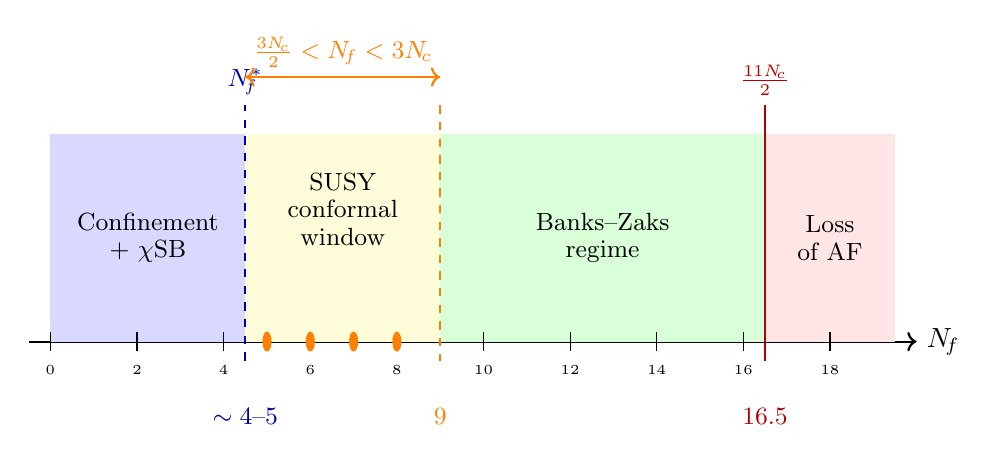
\begin{tikzpicture}[xscale=0.55,yscale=1.2]
  % Axis
  \draw[->,thick] (-0.5,0) -- (20,0) node[right] {$\Nf$};

  % Regions with fills
  \fill[blue!15] (0,0) rectangle (4.5,2.2);
  \fill[yellow!15] (4.5,0) rectangle (9,2.2);
  \fill[green!15] (9,0) rectangle (16.5,2.2);
  \fill[red!10] (16.5,0) rectangle (19.5,2.2);

  % Boundary lines
  \draw[thick,dashed,blue!70!black] (4.5,-0.2) -- (4.5,2.5)
    node[above] {\small $\Nf^*$};
  \draw[thick,dashed,orange] (9,2.5) -- (9,-0.2);
  \draw[thick,red!70!black] (16.5,-0.2) -- (16.5,2.5)
    node[above] {\small $\frac{11\Nc}{2}$};

  % Region labels
  \node[align=center] at (2.25,1.1) {\small Confinement\\[-2pt]\small $+$ $\chi$SB};
  \node[align=center] at (6.75,1.4) {\small SUSY\\[-2pt]\small conformal\\[-2pt]\small window};
  \node[align=center] at (12.75,1.1) {\small Banks--Zaks\\[-2pt]\small regime};
  \node[align=center] at (18,1.1) {\small Loss\\[-2pt]\small of AF};

  % SUSY window markers
  \draw[thick,orange,<->] (4.5,2.8) -- (9,2.8);
  \node[above,orange] at (6.75,2.8) {\small $\frac{3\Nc}{2} < \Nf < 3\Nc$};

  % Integer tick marks
  \foreach \x in {0,2,4,6,8,10,12,14,16,18} {
    \draw (\x,-0.1) -- (\x,0.1);
    \node[below] at (\x,-0.15) {\tiny\x};
  }

  % Key Nf values for SU(3)
  \node[below,blue!70!black] at (4.5,-0.6) {\small $\sim 4$--$5$};
  \node[below,orange] at (9,-0.6) {\small $9$};
  \node[below,red!70!black] at (16.5,-0.6) {\small $16.5$};

  % SUSY window dots
  \foreach \x in {5,6,7,8} {
    \fill[orange] (\x,0) circle (3pt);
  }
\end{tikzpicture}
\caption{Phase diagram of $\SU{3}$ gauge theory as a function of $\Nf$
  (Dirac flavours).  Orange dots mark the SUSY conformal window integers
  $\Nf = 5,6,7,8$.  The non-SUSY lower boundary $\Nf^*$ is
  model-dependent.}
\label{fig:ex-phase-diagram}
\end{figure}

\textbf{(i) $\Nf = 0$: Pure Yang--Mills.}

The theory has no matter fields.  $\bzero = 11 > 0$: strongly asymptotically
free.  The \IR{} is confining with a mass gap $\sim \Lambda_{\QCD}$.
There are no global flavour symmetries, so anomaly matching is vacuous.
The spectrum consists of massive glueballs.

\textbf{(ii) $\Nf = 1,\ldots,\sim 4$: Confinement with chiral symmetry
breaking.}

$\bzero > 0$ (AF), the coupling grows in the \IR, and the theory confines.
The classical global symmetry $\SU{\Nf}_L \times \SU{\Nf}_R \times
\UU{1}_B$ is spontaneously broken:
\[
  \SU{\Nf}_L \times \SU{\Nf}_R \to \SU{\Nf}_V,
\]
producing $\Nf^2 - 1$ massless Goldstone bosons (pions).

't~Hooft anomaly matching constrains the \IR{} spectrum: the anomaly
coefficients (computed in Problem~2 for $\Nf = 2$ and Problem~3 for
general $\Nf$) must be matched by the massless fermions in the confined
phase.  For $\Nf = 2$, the nucleon doublet provides the matching.

\textbf{(iii) $\Nf \approx 5$--$8$ (SUSY conformal window for $\SU{3}$):}

In the SUSY theory, the exact result is that $\Nf = 5,6,7,8$ lie in the
conformal window $3\Nc/2 < \Nf < 3\Nc = 9$.  The theory flows to an
interacting superconformal fixed point in the \IR.  There is no confinement,
no chiral symmetry breaking, and no mass gap.

Anomaly matching is automatically satisfied at the conformal fixed point:
both the \UV{} (free) and \IR{} (interacting CFT) descriptions have the
same massless particle content (the theory is scale-invariant, not confining).

For the \emph{non-SUSY} theory, the situation is uncertain: the lower
boundary $\Nf^*$ of the non-SUSY conformal window is model-dependent,
with estimates ranging from $\sim 8$ to $\sim 12$ for $\SU{3}$.

\textbf{(iv) $\Nf \approx 9$--$16$: Banks--Zaks regime.}

$\bzero > 0$ (AF) and the two-loop coefficient $\bone < 0$ for $\Nf$
sufficiently large.  The theory flows to a Banks--Zaks fixed point at
$\alphas^* = -2\pi\bzero/\bone$.  Near $\Nf = 16$, the fixed point
coupling is small and perturbatively reliable (Problem~2).  As $\Nf$
decreases toward $\Nf^*$, the coupling at the fixed point grows and
eventually the perturbative description breaks down.

\textbf{(v) $\Nf \geq 17$: Loss of asymptotic freedom.}

$\bzero \leq 0$: the coupling is irrelevant in the \UV{} and the theory
is \IR{} free (trivial).  There is no interacting fixed point.  The theory
is not confining and has no interesting strong-coupling dynamics.  It
behaves like QED at low energies.

\medskip

\textbf{(c) Relevance to the dualised SM programme.}

The conformal window is central to the dualised Standard Model because:

\begin{enumerate}[label=\arabic*.]
  \item \textbf{Seiberg duality operates in the conformal window.}
    In SQCD, theories with $3\Nc/2 < \Nf < 3\Nc$ have both an
    ``electric'' description (gauge group $\SU{\Nc}$, strongly coupled
    in the \IR) and a ``magnetic'' description (gauge group
    $\SU{\Nf - \Nc}$, weakly coupled in the \IR).  These are dual
    descriptions of the \emph{same} physics.

  \item \textbf{The SM could be the magnetic dual.}
    If the SM gauge sectors arise as the magnetic (weakly coupled) dual of
    a strongly-coupled electric theory, then the matter content we observe
    (quarks, leptons, Higgs) would be the magnetic ``quarks'' and ``mesons''
    of the dual theory.  This requires the electric theory to lie in or
    near the conformal window.

  \item \textbf{Analytical control.}  Within the conformal window, both
    sides of the duality are under analytical control.  Anomaly matching
    provides exact constraints on the duality map.  This is far more
    powerful than attempting to study the non-SUSY conformal window, where
    no exact results are available.
\end{enumerate}

\textbf{(d) Challenge: $\SU{3}$ with $\Nf = 12$.}

The theory with $\Nf = 12$ is at the heart of the debate about the non-SUSY
conformal window.  At two loops:
\begin{align}
  \bzero &= (33 - 24)/3 = 3, \\
  \bone &= (306 - 12 \times 38)/3 = (306 - 456)/3 = -50, \\
  \alphas^* &= -2\pi \times 3/(-50)
  = 6\pi/50 = 3\pi/25 \approx 0.38.
\end{align}

This value $\alphas^* \approx 0.38$ is \emph{not} small---the perturbative
two-loop result is unreliable.  We are deep in the non-perturbative regime,
and the two-loop beta function cannot be trusted to determine whether the
theory confines or flows to a fixed point.

\textbf{Why lattice simulations are needed:}
\begin{enumerate}[label=\arabic*.]
  \item No perturbative or analytical method can determine whether
    $\alphas^* \approx 0.38$ corresponds to a true fixed point or is an
    artifact of the two-loop truncation.
  \item The SUSY exact result does not apply ($\Nf = 12$ is above the
    SUSY window $\Nf < 9$ for $\SU{3}$, and this is a non-SUSY theory).
  \item Only a non-perturbative method (lattice gauge theory) can
    definitively determine the \IR{} behaviour.
\end{enumerate}

\textbf{Current lattice evidence (summary):}
\begin{itemize}
  \item \textbf{Evidence for conformality:} Some lattice studies
    (notably the LatKMI collaboration) find that the mass spectrum
    scales consistently with a conformal IR fixed point, with a slowly
    running coupling consistent with approximate scale invariance.
  \item \textbf{Evidence for confinement:} Other studies find a
    non-zero chiral condensate and a non-zero string tension, suggesting
    confinement with chiral symmetry breaking.
  \item \textbf{The difficulty:} Near the conformal window boundary,
    the coupling runs very slowly (``walking'').  This makes it hard to
    distinguish between true conformality and very slow running toward
    confinement.  Finite-volume and finite-lattice-spacing effects are
    significant and hard to control.
\end{itemize}

\textit{The bottom line:} The question of whether $\SU{3}$ with $\Nf = 12$
is inside or outside the conformal window remains open as of 2027.  This
uncertainty is one motivation for the dualised SM programme: by working
within the \emph{SUSY} conformal window (where the boundaries are exact),
one avoids this ambiguity entirely.
\end{proof}

\bigskip

\begin{center}
\rule{0.6\textwidth}{0.4pt}

\textit{End of Exercise Set 2.  The conformal window and anomaly matching
from Exercise Sets 1--2 provide the foundation for Seiberg duality
(Lecture~3) and the dualised Standard Model construction (Lectures~6--7).}
\end{center}

%% ========================================================================
%%  BIBLIOGRAPHY
%% ========================================================================
\begin{thebibliography}{99}
\bibitem{BanksZaks1982}
  T.~Banks and A.~Zaks, ``On the phase structure of vector-like gauge
  theories with massless fermions,'' Nucl.\ Phys.\ B \textbf{196} (1982) 189.

\bibitem{Seiberg1995}
  N.~Seiberg, ``Electric--magnetic duality in supersymmetric non-Abelian
  gauge theories,'' Nucl.\ Phys.\ B \textbf{435} (1995) 129
  [hep-th/9411149].

\bibitem{DeGrand2015}
  T.~DeGrand, ``Lattice tests of beyond Standard Model dynamics,''
  Rev.\ Mod.\ Phys.\ \textbf{88} (2016) 015001 [arXiv:1510.05018].

\bibitem{PS1995}
  M.~E.~Peskin and D.~V.~Schroeder, \textit{An Introduction to Quantum
  Field Theory}, Addison-Wesley, 1995.

\bibitem{Sannino2024}
  F.~Sannino \textit{et al.}, ``Dualised Standard Model,''
  arXiv:2407.17281 [hep-ph].
\end{thebibliography}

\end{document}
